\documentclass[12pt,oneside,a4paper]{article}

\usepackage[backend=biber,style=numeric, sorting=none]{biblatex}
\usepackage{xcolor}
\usepackage{todonotes}
\usepackage{amsmath}
\usepackage{multicol}
\usepackage{caption}
\usepackage{hyperref}
\usepackage{graphicx}
\usepackage{listings}
\usepackage[margin=1.35in]{geometry}

\lstdefinestyle{bsvstyle}{
	backgroundcolor=\color{backcolour},   
	numberstyle=\tiny\color{gray},
	basicstyle=\ttfamily\footnotesize,
	breakatwhitespace=false,         
	breaklines=true,                 
	captionpos=b,                    
	keepspaces=true,                 
	numbers=left,                    
	numbersep=5pt,                  
	showspaces=false,                
	showstringspaces=false,
	showtabs=false,                  
	tabsize=2
}

\lstdefinelanguage{BSV}{
	keywords={rule, Vector,typedef, enum, int, String, Reg, Bit, begin, end, endrule, method, endmethod, Action, interface, endinterface, module, endmodule, Reg\#, Bool, let, True, False},
	keywordstyle=\color{codeblue}\bfseries,
	ndkeywords={import, if, else, return, deriving},
	ndkeywordstyle=\color{codepurple}\bfseries,
	identifierstyle=\color{black},
	sensitive=false,
	comment=[l]{//},
	morecomment=[s]{/*}{*/},
	commentstyle=\color{codegreen}\ttfamily,
	stringstyle=\color{red}\ttfamily,
	morestring=[b]',
	morestring=[b]"
}

\definecolor{codegreen}{RGB}{14, 161, 70}
\definecolor{codeblue}{RGB}{43, 45, 179}
\definecolor{codepurple}{RGB}{196, 53, 178}
\definecolor{backcolour}{RGB}{217, 217, 217}

\lstset{
	language=BSV,
	style=bsvstyle
}

\DeclareCaptionFormat{listing}{\rule{\dimexpr\textwidth\relax}{0.4pt}\par\vskip1pt#1#2#3}
\captionsetup[lstlisting]{format=listing,singlelinecheck=false, margin=0pt,labelsep=space,labelfont=bf}

\usepackage{booktabs}
\usepackage[noabbrev,capitalise]{cleveref}
\crefname{listing}{snippet}{snippet}
\Crefname{listing}{Algorithm}{Algorithms}
\renewcommand\lstlistingname{Code snippet}
\def\lstlistingcrefname{snippet}
\usepackage{url}

\addbibresource{biblio.bib}

\title{\textbf{RISC-V processors with BSV}}

\author{High Performance Processors and System\\ A.Y. 2020/2021\\\\\\\\\\\Large R\normalsize ICCARDO \Large N\normalsize ANNINI\\}

\date{\parbox{\linewidth}{\centering%
		\today\endgraf\bigskip\bigskip\bigskip\bigskip\bigskip\bigskip\bigskip
		\large T\normalsize UTORS\endgraf\medskip \normalsize E\footnotesize MANUELE \normalsize D\footnotesize EL \normalsize S\footnotesize OZZO \endgraf\smallskip
		\normalsize D\footnotesize AVIDE \normalsize C\footnotesize ONFICCONI \endgraf\bigskip\bigskip\bigskip
		\large P\normalsize ROFESSOR\endgraf\medskip \normalsize M\footnotesize ARCO \normalsize D\footnotesize OMENICO \normalsize S\footnotesize ANTAMBROGIO 
		}}
\begin{document}

\begin{titlepage}
	\centering
	\clearpage
	\maketitle
	\thispagestyle{empty}
	\vspace*{1cm}
	\vfill
	\centering
	
\includegraphics{logo_polimi.png}
\includegraphics{logo_NECST.png}
\end{titlepage}

\tableofcontents
\newpage

\begin{abstract}
Bluespec System Verilog (\textbf{BSV}) is a state-of-the-art Hardware Description Language.
Bluespec compilation toolchain (\textbf{BSC}) has been recently released as open source \cite{bsc}. The goal of the project was investigating the potentiality of said toolchain implementing different \textbf{RISC-V} processors of increasing complexity.\\
\end{abstract}

\section{Introduction} \label{sec:intro}

This report covers chronologically the path that I have followed during the development of this project.
 
It starts from a quick overview on the \textit{RISC-V} ISA, focused on the key ingredients that make this ISA one of the most trend topics in Computer Engineering.

It proceeds with the analysis of the \textit{Bluespec System Verilog} language, outlining its novelties with respect to other hardware description languages, as well as its main features and capabilities. 

The last section is devoted to the development of various RISC-V processor designs, describing in details the characteristics of each processor and motivating the various design choices, starting from a one cycle non pipelined processor and ending with a 6 stage pipelined one enriched with multiple branch predictors.

Everything I have produced within this project (code, scripts, this report itself) is available on GitHub \url{https://github.com/riccardo-nannini/BSV_RISC-V}


\section{RISC-V} \label{sec:risc-v}
\subsection{What is RISC-V}
Since the processor designs will be based on RISC-V, knowing this ISA is fundamental.

Born in 2010 at UC Berkeley by the work of graduate students Andrew Waterman, Yunsup Lee and professors David Patterson, Krste Asanovic \cite{risc-v_original}, RISC-V was built with the experience gained from the four previous major RISC ISA design from UC Berkeley (thus justifying the ‘V’).

As the name suggests, RISC-V belongs to the family of \textbf{RISC} ISAs. In particular, RISC instruction sets are characterized by \textit{small} and \textit{highly optimized} instructions that ease \textit{pipeline} implementation, along with a large number of \textit{general purpose registers}. 

RISC-V, like many other RISC ISAs, is a \textbf{load-store architecture}; this means that, apart from some exceptions, arithmetic and logic instructions operate on register and not on memory directly. Load and store instructions take care of the transit of data from memory to register and vice versa.
\subsection{Instructions set goals}
When the first paper that declared the birth of RISC-V \cite{risc-v_original} was released back in 2011, the authors stated some of the goals that they wanted to achieve when designing this instructions set. In particular the main objectives include, but are not limited to:
\begin{itemize}
	\item Provide a \textit{realistic} but \textit{open} ISA, suitable for direct hardware implementation
	\item Provide a \textbf{small} but \textbf{complete} ISA, that avoids "\textit{over-architecting}" for a particular microarchitecture style or implementation technology.
	\item Support highly-parallel multicore implementations, including heterogeneous multiprocessors
	\item Support an efficient dense \textit{instruction encoding} with variable-length instructions (generally typical of CISC ISAs).
	\item \textbf{base-plus-extension}: provide a set of standard but optional extensions.
\end{itemize}
In order to achieve these goals many design choices were taken, sometimes in line with other similar ISAs, sometimes with unusual decisions.

\subsection{Main features}
RISC-V has 2 base variants, \textbf{RV32} and \textbf{RV64}, providing 32-bit or 64-bit user-level address spaces respectively. A 128-bit extension is available but mostly aimed at the future of warehouse scale computing.
\subsubsection{Registers}
RISC-V uses 31 general-purpose registers  {\fontfamily{cmtt}\selectfont{x1-x31}} with  {\fontfamily{cmtt}\selectfont{x0}} hardwired to the costant 0. Moreover, 32 64-bit registers {\fontfamily{cmtt}\selectfont{f0-f31}} holding single or double-precision floating-point values are available.

There are also two special registers: the \textit{program counter} {\fontfamily{cmtt}\selectfont{pc}} holds the address of the current instruction while the \textit{floating point status register} {\fontfamily{cmtt}\selectfont{fsr}} contains the operating mode and exception status of the floating-point unit.
\subsubsection{Instruction encoding}
In addition to standard fixed-length 32-bit instructions, RISC-V supports extensions with \textbf{variable-length} ones too, useful in reducing code size specially for specific domains like embedded systems.

\cref{riscv:encoding} shows the instruction length encoding convention. 32-bit instructions have the 2 least significant bits always set to {\fontfamily{cmtt}\selectfont{1}} while the 16-bit ones must have said bits in any combination but {\fontfamily{cmtt}\selectfont{11}}.
Instructions longer than 32-bits have additional lower bits set to {\fontfamily{cmtt}\selectfont{1}}.\medskip

\begin{figure}[h]
	\centering
	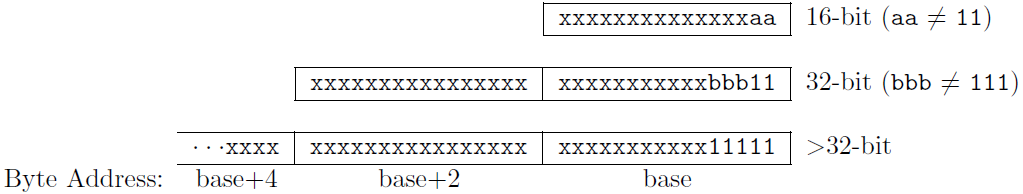
\includegraphics[scale=0.65]{risc-v_encoding}
	\caption{RISC-V instruction encoding}
	\label{riscv:encoding}
\end{figure}

\subsubsection{Instruction format}
Six basic instruction formats are present in the base version of the ISA as shown in \cref{riscv:format}.

\begin{figure}[h]
	\centering
	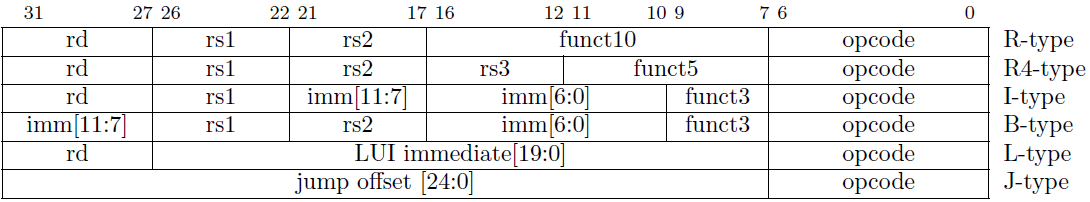
\includegraphics[scale=0.65]{risc-v_format}
	\caption{RISC-V instruction formats}
	\label{riscv:format}
\end{figure}

It is worth underlining a particular design choice made by the authors. Since, as they state, the \textit{decoding} of register specifiers is usually on the \textbf{critical path} in implementations, they decided to keep all register specifiers in the same position across every instruction type. This comes with the tradeoff of having some instructions with an immediate value that has to be split in two parts.

\textbf{R-Type} instructions are for operations with two source registers (\textit{rs1} and \textit{rs2}) while \textbf{R4-Type} format is for special three source register floating point instructions. Moreover, \textbf{I-Type} format is for operations between a source register (\textit{rs1}) and an 12-bit sign-extended immediate, while \textbf{B-Type} instructions are designed for conditional branches (where the branch type is specified in \textit{funct3}).
The LUI (\textit{Load upper immediate}) operation, generally used to build 32-bit constants, is the typical instruction specified by the \textbf{L-Type}, meanwhile \textbf{J-Type} instructions encode a 25-bit target address as a PC-relative offset.

Describing in details the specification of every instruction is way out of the focus of this report and is already done with great details in the original paper \cite{risc-v_original}.\\

In the end, just a mention to the \textit{fsr}, a special register containing the status of floating-point operation, shown in \cref{riscv:fsr}.

\begin{figure}[h]
	\centering
	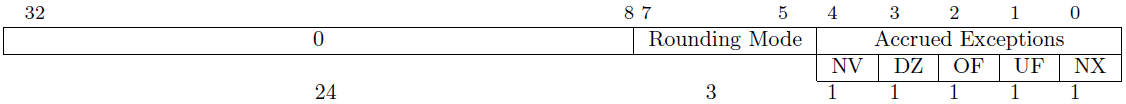
\includegraphics[scale=0.575]{risc-v_fsr}
	\caption{Floating-point status register}
	\label{riscv:fsr}
\end{figure}

It makes possible to specify the rounding mode with a specific encoding as well as reading the status of the previous floating-point operation in the flag bits.\\
\subsection{License}
Until here the main features of RISC-V were summarized.
Despite being a really well designed standard, this by itself does not explain the popularity of this ISA.

In fact, one of the main factor of his success is that RISC-V is provided under a \textbf{free open source} license that does not require fees to use.

This is quite unusual in the instruction set architectures world, that for a great majority are \textit{proprietary} due to historical or business reasons. Companies like ARM, IBM and Intel have patents on their ISAs which prevent others from using them without licenses.

Negotiations for said licenses can take 6-24 months and can cost up to \$1M-\$10M, ruling out academia and other with small volumes. An ARM license, for instance, doesn't even let you design an ARM core; you just get to you \textit{their} designs \cite{risc-v_free}.

Some open-source ISA already existed but were not as popular and well designed as RISC-V is.

The birth of this standard enabled a \textbf{real free open market} of processor designs leading to:
\begin{itemize}
	\item greater innovation via \textbf{free-market competition}
	\item shared open core designs
	\item processors becoming \textbf{affordable} for more devices
\end{itemize}

\section{BSV}
The hardware description language used to implement the RISC-V processors within the project is \textbf{Bluespec System Verilog} (BSV).

Belonging to Bluespec Inc, co-founded in 2003 by MIT professor Arvind, the BSV language is aimed at providing hardware designers used to Verilog, VHDL or System Verilog, a \textbf{high level} language for hardware design and synthesis.

Based on a synthesizable subset of SystemVerilog, BSV can significantly improve the hardware design process with some key innovations: 

\begin{itemize}
	\item Hardware behavior is expressed with \textbf{Rules}.
	Rules are powerful concepts for achieving correct concurrency and eliminating race conditions.
	\item \textbf{Polymorphism} makes possible to write more general code and reuse designs and glue them together in a flexible way.
	\item Provides \textbf{formal semantics}, enabling formal verification and formal design-by-refinement. This is due to the fact that BSV rules are based on \textit{Term Rewriting Systems}, a clean formalism supported by decades of theoretical research in the computer science community.
\end{itemize}

\subsection{General overview}

This section is devoted to the main features of BSV in order to give the reader a general overview of the language and understand its strength. The complete reference guide (also used for this quick introduction) can be found at \cite{bsv_guide}.
\subsubsection{Modules and interfaces}
In order to understand BSV, it is useful to start with the notion of \textbf{modules} and \textbf{interfaces}, the core of the language. Modules and interfaces are what, in the end, is turned into actual hardware. 

An interface describes what a module 'offers' to the outside. On the other hand, a module 'implements' its interface as it prefers.

In BSV, an interface consists of \textit{methods} that encapsulate the possible transactions that clients can perform. 

\begin{lstlisting}[label={list:moduleinterface},caption={Example of module and interface}]
interface Fifo#(int n);	//n is the size of the fifo

	method Action enqueue(Bool x);
	method Action dequeue;
	method Bit#(8) first;
	
endinterface

module mkFifo( Fifo#(n) );

	//... implementation
	
endmodule
\end{lstlisting}

When it comes to modules, however, we need to distinguish between a module \textit{definition} and a module \textit{instantiation}. A module definition is like a class in object oriented programming while a module instantiation can be considered as an object of said class.

A module consists of three things: 
\begin{itemize}
	\item a \textbf{state}
	\item  \textbf{rules} that operate on that state
	\item an \textbf{interface} to the outside world
\end{itemize}
\subsubsection{State}
In Verilog and SystemVerilog, one simply declares a variable, and a synthesis tool "infers" how those variable actually map into state element in hardware; a variable may map into a bus, a latch, a flip-flop or even nothing.

BSV eliminates this ambiguity and places the state control directly in the hand of the designer. BSV \textit{never} implies state; variables are just convenient names for intermediate values.

State components are declared (and instantiated) after the module declaration like in \cref{bsv:state}

\begin{lstlisting}[label={bsv:state},caption={Example of state declaration}]
module mkFifo( Fifo#(n) );

    Vector#(n, Reg#(Bit#(8))) data <- replicateM(mkRegU());
		Reg#(Bit#(8)) 	  	 value_reg <- mkReg(0);
		
		//...

endmodule
\end{lstlisting}

\subsubsection{Types and polymorphism}

Every variable and every expression in BSV has a \textit{type}.
BSV supports standard \textit{simple type} like in \cref{bsv:simpletype}
\begin{lstlisting}[label={bsv:simpletype},caption={Simple types}]
int
Bool
String
\end{lstlisting}
or \textit{parametrized} types (either standard or user-defined)in the form of {\fontfamily{cmtt}\selectfont{\textbf{X\#}}(t\textsubscript{1},..., t\textsubscript{n})}
\begin{lstlisting}[label={bsv:paramtype},caption={Parametrized types}]
Tuple2#(int, Bool)		//pair of items, an int and a Bool
List#(Bool)					  //list of booleans
Vector#(n, int)				//vector of n integers
Bit#(16)							//16-bit wide bit-vector
Int#(29)							//signed integer, 29 bits wide
Vector#(16, List#(Int#(29)))	//vector of 16 Lists of 29 bits wide signed integers
\end{lstlisting}

In \cref{bsv:paramtype} it is possible to observe that parametrized types utilize \textbf{polymorphism}, making code way more reusable.

It is worth mentioning also the type \textbf{Action} that denotes any expression that acts on the \textit{state} of the circuit, fundamental in order to produce useful hardware.
\subsubsection{Rules}
\textit{Rules} specify the internal behavior of modules. A rule may have a \textit{guard} (boolean expression) that indicates when the rule can execute (fire), and a \textit{body}, of type Action, that describes what the rule does.
\begin{lstlisting}[label={bsv:paramtype},caption={Autoincrementing couter with a single rule}]
module mkCounter(Empty);
	Reg#(Bit#(8)) value <- mkReg(0);
	
	rule increment (value >= 0); //guard
		value <= value + 1;			 	 //body
	endrule
endmodule
\end{lstlisting}

The body of a rule can contain, with an ad-hoc semantic, the basic constructs typical of software programming languages such as if-else, switch, loop etc.

\subsubsection{Dynamic semantic}

The simplest way to understand the dynamic semantic of BSV is thinking that, at each step, the system picks any \textit{one} enabled rule and fires it.

Since only one rule is executed at each step, we have only to look at each rule in \textbf{isolation}, without worrying about the interactions with other rules simultaneously. Each rule can be viewed as an \textbf{atomic state transition}.

The BSC compiler maps BSV into efficient parallel clocked synchronous hardware. In particular, the mapping allows multiple rules to be executed at each clock cycle. The compiler is able do to this by producing a \textbf{role-control circuit} which takes all the enabled conditions and possible data outputs (actions) and feeds them into a \textbf{scheduler} circuit. It is the scheduler duty, at each clock cycle, to select a subset of conflict-free rules to fire.

\section{Processor designs}

This section is devoted to the processor designs created within this project.

After studying the RISC-V ISA and getting to know the BSV language, it was the point to get my hands dirty and creating a variety of processor designs.

Every design, among other things like BSV working examples I have made as an exercise, is available in the GitHub repository \url{https://github.com/riccardo-nannini/BSV_RISC-V}.
\subsection{Starting point}
I was provided with an initial setup comprising a processor infrastructure (\cref{infrastructure}) based on Connectal \cite{connectal}, some test benches, and an initial simple one cycle implementation of a RISC-V processor.

\begin{figure}[h]
	\centering
	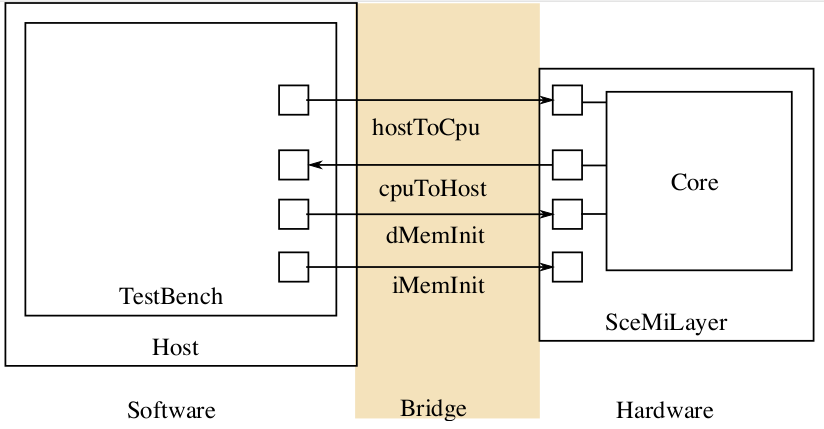
\includegraphics[scale=0.4]{infrastructure.png}
	\caption{Processor infrastructure with control signals}
	\label{infrastructure}
\end{figure}

\cref{onecycle} shows the structure of the initial one cycle processor. 

Starting from here, I developed more realistic processors of increasing complexity. 


\begin{figure}[h]
	\centering
	\includegraphics[scale=0.75]{onecycle.png}
	\caption{One cycle processor architecture}
	\label{onecycle}
\end{figure}

\subsection{Two cycles}
The one cycle processor is able to operate in a single cycle because it has \textbf{separate} instruction and data memory; my first design was aimed at creating a more realistic architecture, based on the von Neumann model, with a single memory accessible only once per clock cycle.

This indeed creates a structural hazard, solved by splitting the instruction execution in \textbf{two cycles}: one for fetching the instruction and one for decoding/executing the instruction and access the memory.

In order to achieve this, an intermediate register ({\fontfamily{cmtt}\selectfont{f2d}}) has to hold the data that a state has to pass to the following one (in this case the fetched instruction).

\begin{figure}[h]
	\centering
	\includegraphics[scale=0.8]{twocycle.png}
	\caption{Two cycles processor architecture}
	\label{twocycle}
\end{figure}

\begin{lstlisting}[label={twocyclecode},caption={Two cycles processor simplified code}]
typedef enum {
	Fetch, Execute
} State;

Reg#(State) state <- mkRegU;

rule doFetch(state == Fetch);      
	f2d <= mem.req(pc);		//fetch instruction
	state <= Execute;			//pass to the execute state
endrule

rule doExecute(state == Execute);
	let instruction = f2d;
	//... decode, execute, memory and writeback
	state <= Fetch;	
endrule
\end{lstlisting}

\subsection{Four cycles}
Another unrealistic assumption I had to get rid of was that, since now, memory access was treated as \textit{combinational}. The processor had only to set some input lines to the memory and receive an answer in the same cycle. Most real memories have reads with \textbf{longer latencies}: first you set the address bits and then the result is ready in the next clock cycle.

This structural hazard is avoided by further splitting the processor into \textbf{4 cycles}:
\begin{itemize}
	\item the \textit{instruction fetch} stage sets the address lines on the memory to read the current instruction.
	\item the \textit{instruction decode} stage reads the instruction from memory, decodes it and reads the registers.
	\item the \textit{execute} stage performs ALU operations, writes data to memory and sets up address lines for load instructions.
	\item the \textit{write back} stage reads the result from memory (if any) and writes the register file.
\end{itemize}

\begin{lstlisting}[label={fourcyclecode},caption={Four cycle processor simplified code}]
typedef enum {
Fetch, Decode, Execute, WriteBack
} State;

Reg#(State) state <- mkRegU;

rule doFetch(state == Fetch);      
	mem.req(pc);			//requests the instruction
	state <= Decode;	//pass to the decode state
endrule

rule doDecode(state == Decode);
	DecodedInst dInst = decode(mem.resp());
	//... reads from registers
	state <= Execute;
endrule

rule doExecute(state == Execute);
	//performs ALU operation and request data if load instruction
	state <= WriteBack;
endrule

rule doWriteBack(state == WriteBack);
	//reads from memory if load and writes back to registers
	state <= Fetch;
endrule
\end{lstlisting}

\subsection{Two-stage pipelined}
In the above-described designs, when the processor was in a particular state, the rest of the hardware remained unused. A \textbf{pipeline} approach is aimed at improving performance by parallelizing instructions execution. This, however, brings up \textbf{data} and \textbf{control hazards} that we ignored up to now. In order to make a step at the time, I started with a \textbf{two-stage pipelined} processor (bringing back the good old unrealistic combinational reads) that rules out data hazards (read registers, execution and write-back done in the same clock cycle).\\

While the stage structure is similar to the two clock design (fetch/decode in one stage, execute/memory/writeback in the second), we need some form of \textbf{next instruction prediction} (the fetch stage has to fetch the instruction before the previous one has terminated) and a way to kill wrong path instructions in case of a \textbf{misprediction}.

This can be achieved by using a  {\fontfamily{cmtt}\selectfont{FIFO}} queue as an intermediate register between the stages and, in case of a misprediction, clear said  {\fontfamily{cmtt}\selectfont{FIFO}} (as it contains a wrong-path instruction) and redirect the {\fontfamily{cmtt}\selectfont{pc}} with the correct address. This pc-overwriting action is possible due to  {\fontfamily{cmtt}\selectfont{EHR}} (\textit{Ephemeral History Register}), an hardware structure that allows to have multiple writes with different 'priorities'.

\begin{figure}[h]
	\centering
	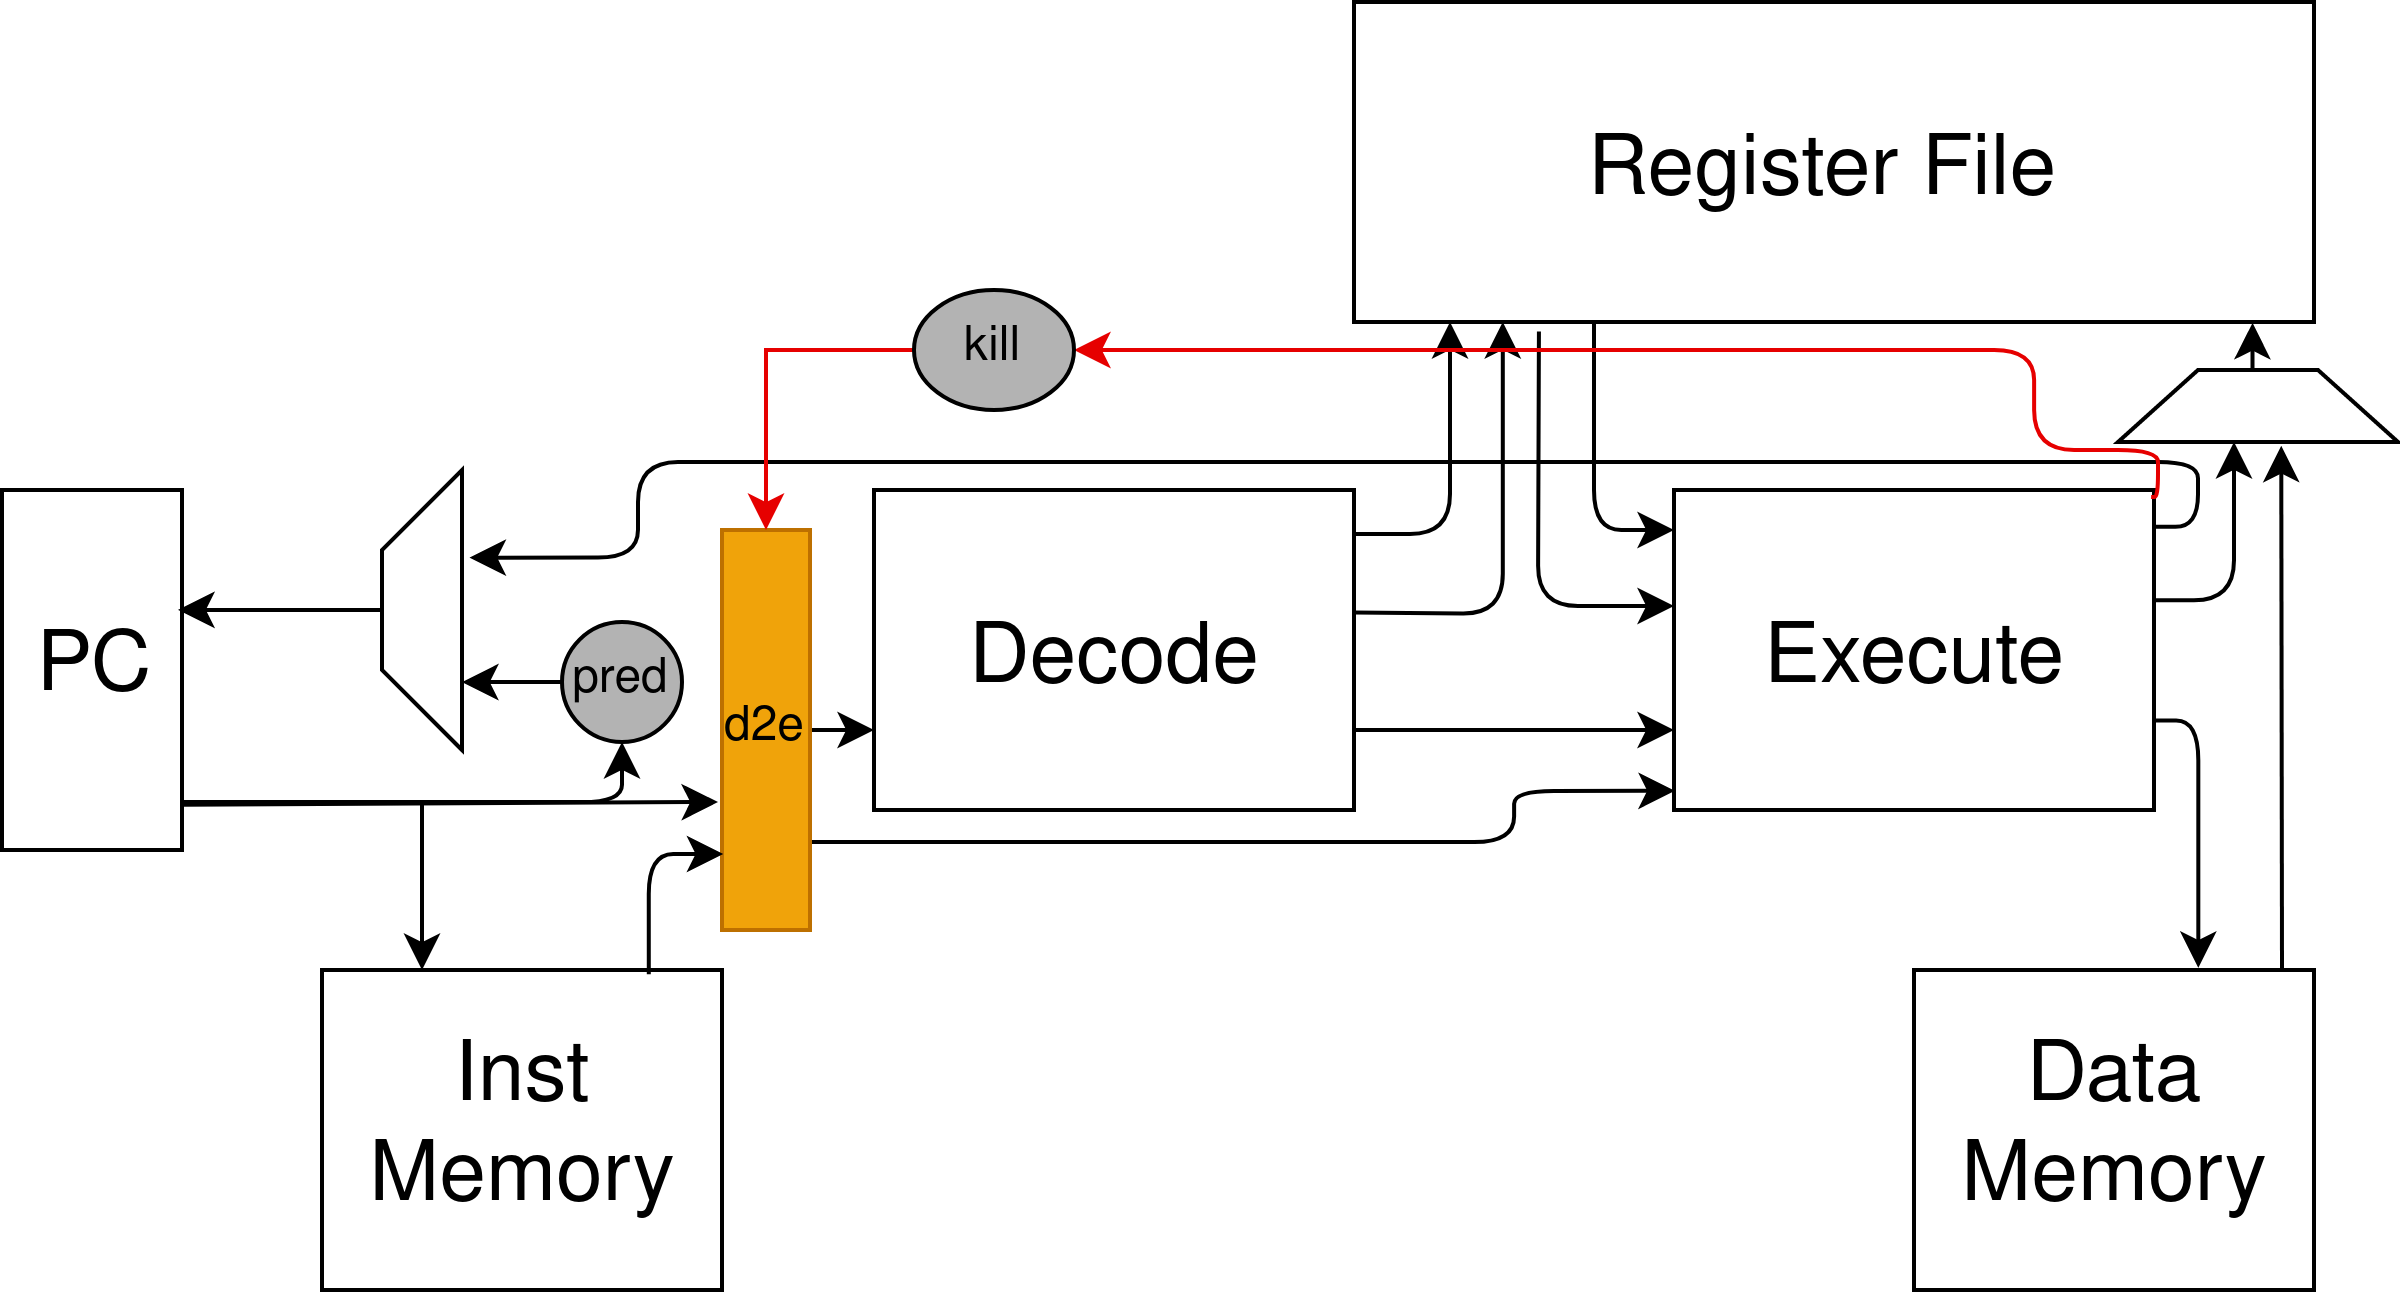
\includegraphics[scale=0.9]{twoStage.png}
	\caption{Two stage pipelined processor architecture}
	\label{twostage}
\end{figure}
\subsubsection{Next address prediction}
The next instruction prediction can be carried out in multiple ways. At first I used a simple {\fontfamily{cmtt}\selectfont{pc+4}} as a predictor for this design and then replaced it in a second moment with a {\fontfamily{cmtt}\selectfont{BTB}} (\textit{Branch Target Buffer}), a cache storing the target address for the next instruction after a branch. In the fetch stage the  {\fontfamily{cmtt}\selectfont{BTB}} is accessed using the n lowest bit of the current pc as an index to the cache. If an entry for the  {\fontfamily{cmtt}\selectfont{pc}} is present it is selected as the next  {\fontfamily{cmtt}\selectfont{pc}}, otherwise {\fontfamily{cmtt}\selectfont{pc+4}} is chosen.

\cref{btbbench} shows the different performance of the design when using a {\fontfamily{cmtt}\selectfont{BTB}} with respect to a plain pc + 4 predictor.

\begin{figure}[h]
	\centering
	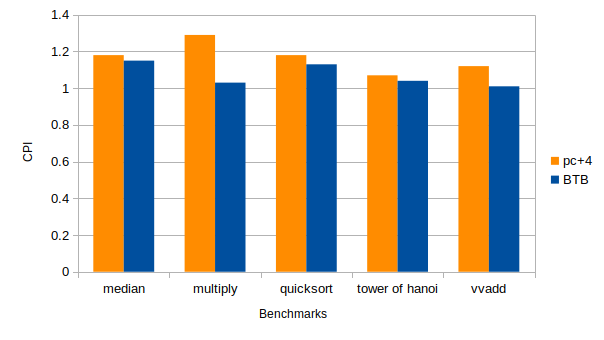
\includegraphics[scale=0.7]{predbtb}
	\caption{CPI comparison with different benchmarks}
	\label{btbbench}
\end{figure}

\subsection{Six stage pipelined}
For the last design I have implemented a six stage pipelined processor, getting rid of combinational reads of the two stage one.

This, however, creates the possibility of having data hazards. Since the execution will be in-order, the only hazard we should take care of are \textbf{RAW} (Read After Write); an instruction might read a register that would have been written by a previous instruction that has not committed yet.\\

In this design I solved this type of conflict using {\fontfamily{cmtt}\selectfont{scoreboard}}. 
{\fontfamily{cmtt}\selectfont{Scoreboard}} is a data structure for \textit{centralized hazard management} that keeps track of the registers currently involved in the pipelined instructions. 

Every instruction goes through the {\fontfamily{cmtt}\selectfont{scoreboard}}: if no conflict are found the instruction proceeds in the pipeline and the used registers are saved in the  {\fontfamily{cmtt}\selectfont{scoreboard}}; if a conflict is found, the instruction stalls.

\begin{lstlisting}[label={fourcyclecode},caption={Scoreboard integration in the pipeline}]
Scoreboard#(10)   sb <- mkCFScoreboard;

rule doRegisterFetch();      
	if (!sb.search1(inst.src1) && !sb.search2(inst.src2))	
	//search if the operand register are present in the scoreboard
		begin	sb.insert(inst.dst);	
		//...
		end
	else
		// STALL
endrule

rule doWriteBack();
	sb.remove		//removes the instruction from scoreboard
endrule
\end{lstlisting}

The six stage pipeline is divided in the following stages:
\begin{itemize}
	\item \textbf{Instruction fetch}: requests instruction from memory and updates PC using the BTB.
	\item \textbf{Decode}: receives instruction from memory and decodes it.
	\item \textbf{Register fetch}: reads from register file.
	\item \textbf{Execute}: executes the instruction and corrects mispredictions.
	\item \textbf{Memory}: sends memory requests for load/store.
	\item \textbf{Write back}: receive responses and writes to register file.
\end{itemize}
The processor needs an intermediate {\fontfamily{cmtt}\selectfont{FIFO}} queue between each stage carrying the necessary information forward.

\subsubsection{BHT}
In order to further improve branch prediction I have implemented and integrated a \textbf{2-bit BHT} (\textit{Branch History Table}). It is a table with 2 bits for each entry that are updated based the previous behavior of the branch. By checking said bits, the {\fontfamily{cmtt}\selectfont{BHT}} predicts whether to take or not the branch.

The {\fontfamily{cmtt}\selectfont{BHT}} is accessed in the decode stage (we need to know that the instruction is a branch in order to use the table) and redirects the {\fontfamily{cmtt}\selectfont{pc}}, killing wrong-path instructions, in case the prediction of the {\fontfamily{cmtt}\selectfont{BTB}} was not in line with the decision of the {\fontfamily{cmtt}\selectfont{BHT}}.

\cref{bhtbench} shows how the number of clock cycles per instruction changes in different benchmarks when using the {\fontfamily{cmtt}\selectfont{BHT}} or not.

\begin{figure}[h]
	\centering
	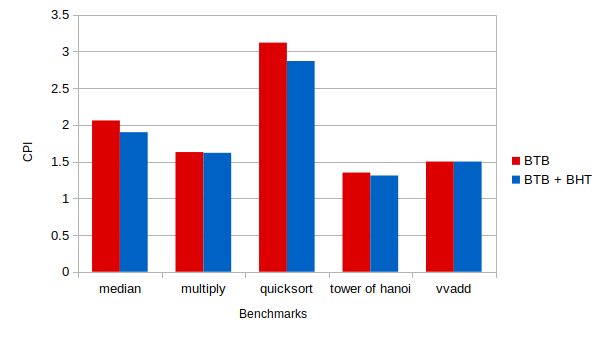
\includegraphics[scale=0.7]{predbhb}
	\caption{CPI comparison with different benchmarks}
	\label{bhtbench}
\end{figure}

\subsubsection{RAS}

As the last improvement to branch predictions I have implemented a \textbf{RAS}. The {\fontfamily{cmtt}\selectfont{Return Address Stack}} is a predictor aimed at improving \textit{Jump register} instructions ({\fontfamily{cmtt}\selectfont{JALR}} and {\fontfamily{cmtt}\selectfont{JAL}}). According to the RISC-V specification, this two types of unconditional jumps save the address of the instruction following the jump ({\fontfamily{cmtt}\selectfont{pc+4}}) in register x1 ({\fontfamily{cmtt}\selectfont{JAL}}) or in  register \textit{rd} specified in the instruction ({\fontfamily{cmtt}\selectfont{JALR}}). Most {\fontfamily{cmtt}\selectfont{JAL}} and {\fontfamily{cmtt}\selectfont{JALR}} instructions found in programs are used to call or return from functions.

The {\fontfamily{cmtt}\selectfont{RAS}}, implemented along with {\fontfamily{cmtt}\selectfont{BHT}} in the decode stage, works by maintaining a stack where return addresses are pushed when a jump calling a routine is found and popping said addresses when another jump instruction returning from a function is detected. Depending on the frequency of jumps in a program, this predictor can slightly improve performances. 



\printbibliography

\end{document}


